\headerbox{\bf\color{sufered} Hessian Sparsification}
{name=hessian-sparsification,column=0,below=contribution,span=2}
{
    Our sparsification scheme is designed based on the structure of the Hessian matrix, which preserves its diagonal elements and symmetry. The impact of this sparsification on the eigenvalues of the Hessian matrix is then analyzed under a \emph{very weak} assumption, leading to the following results:
    \begin{itemize}
        \item \emph{Any} valid sparsification scheme maintains positive definiteness.
        \item The sparsified Hessian matrix is guaranteed to have a smaller condition number. In particular, the biggest eigenvalue is reduced and the smallest eigenvalue is increased.
        \item The assumption is valid for almost \emph{any} sparsification scheme, allowing for highly flexible algorithmic designs and \emph{extremely sparse} matrices.
    \end{itemize}
    The assumption merely requires the existence of a power of the sparsified Hessian matrix in which all entries are strictly positive. A numerical verification is shown below:

    \vspace{0.5em}

    \begin{center}
    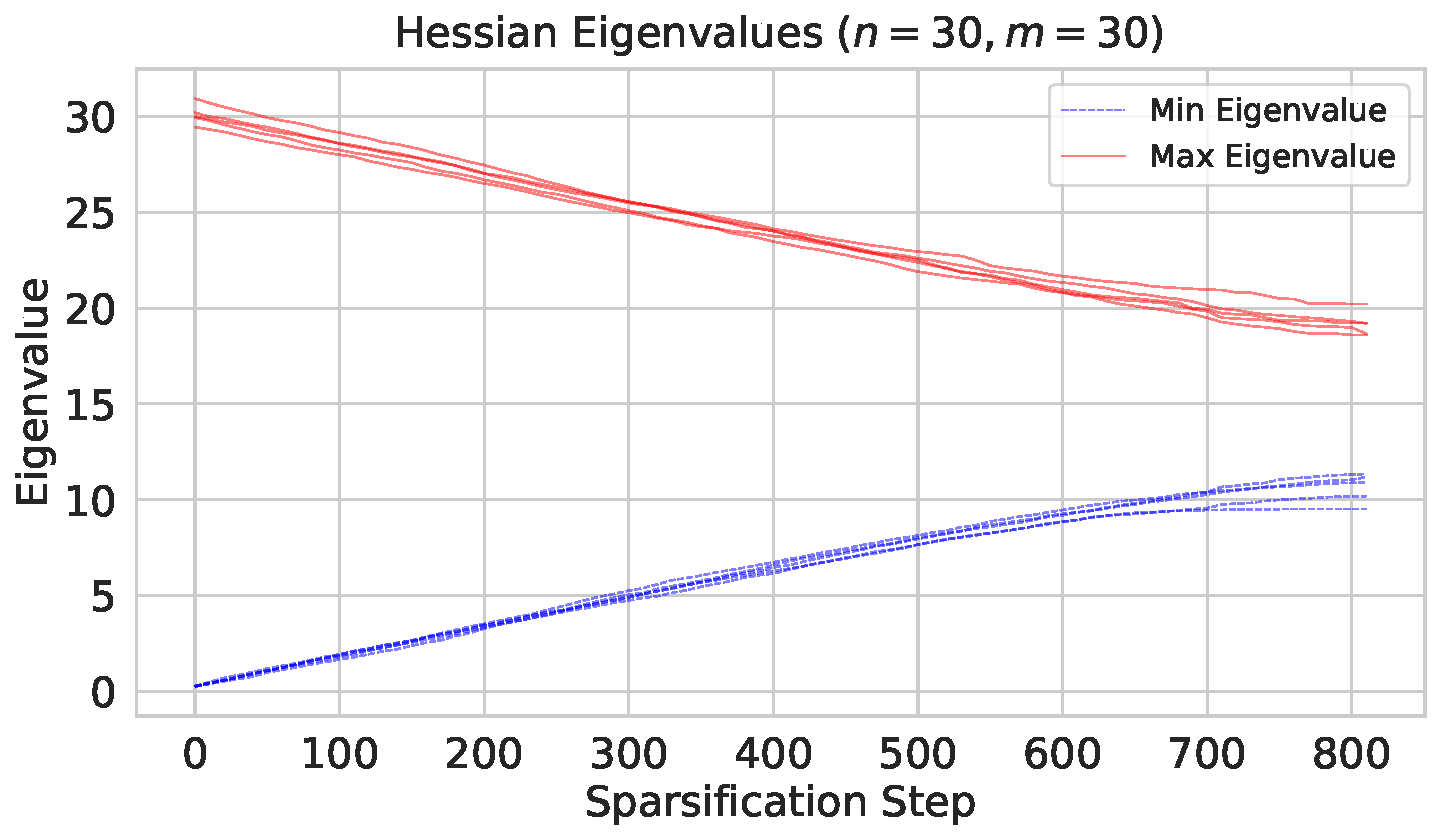
\includegraphics[width=0.48\textwidth]{save/eigen/eigenvalues_n30_m30.pdf}
    \hfill
    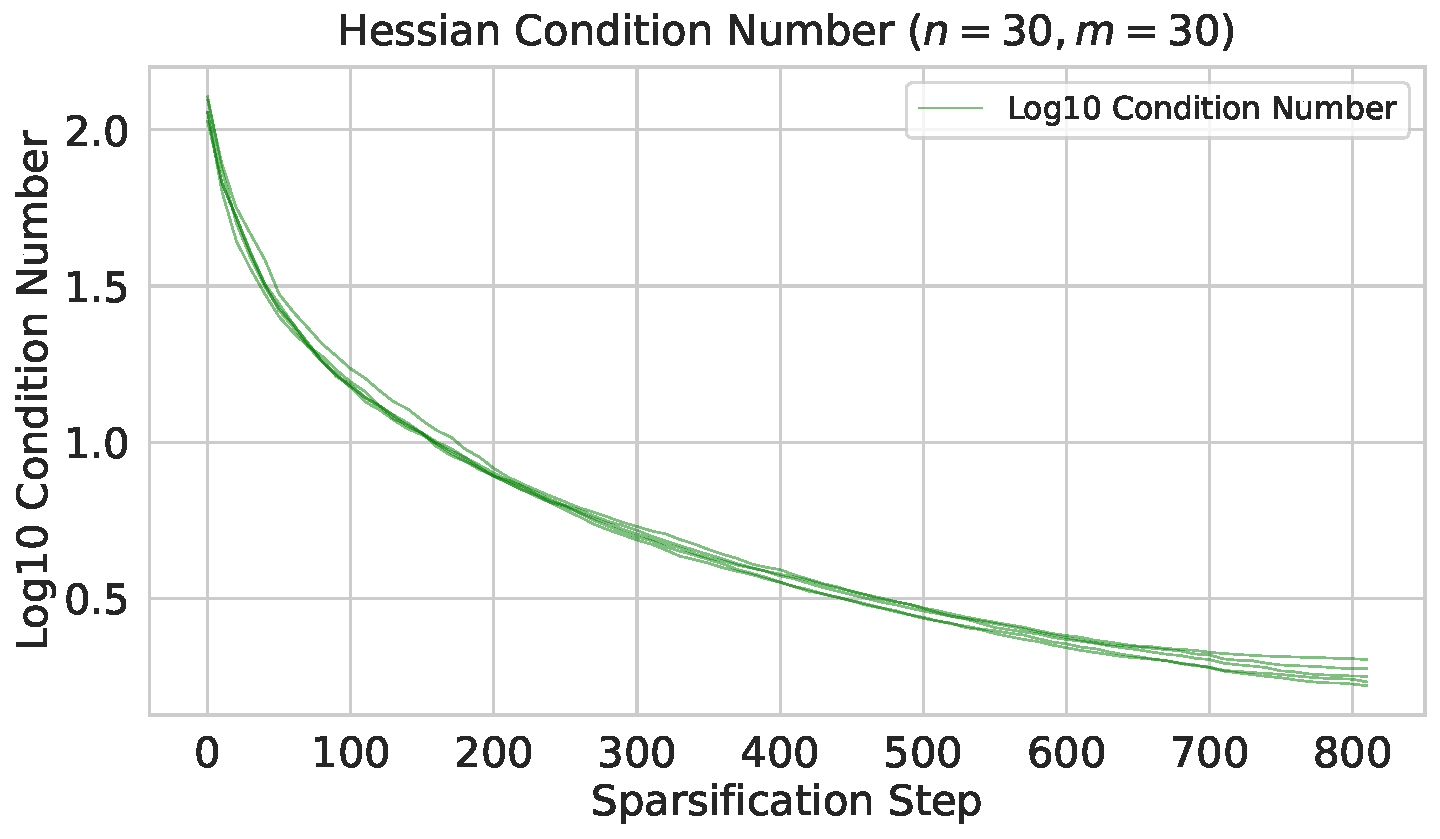
\includegraphics[width=0.48\textwidth]{save/eigen/condition_number_n30_m30.pdf}
    \end{center}
}
